% Created by tikzDevice version 0.12.6 on 2024-07-27 08:35:47
% !TEX encoding = UTF-8 Unicode
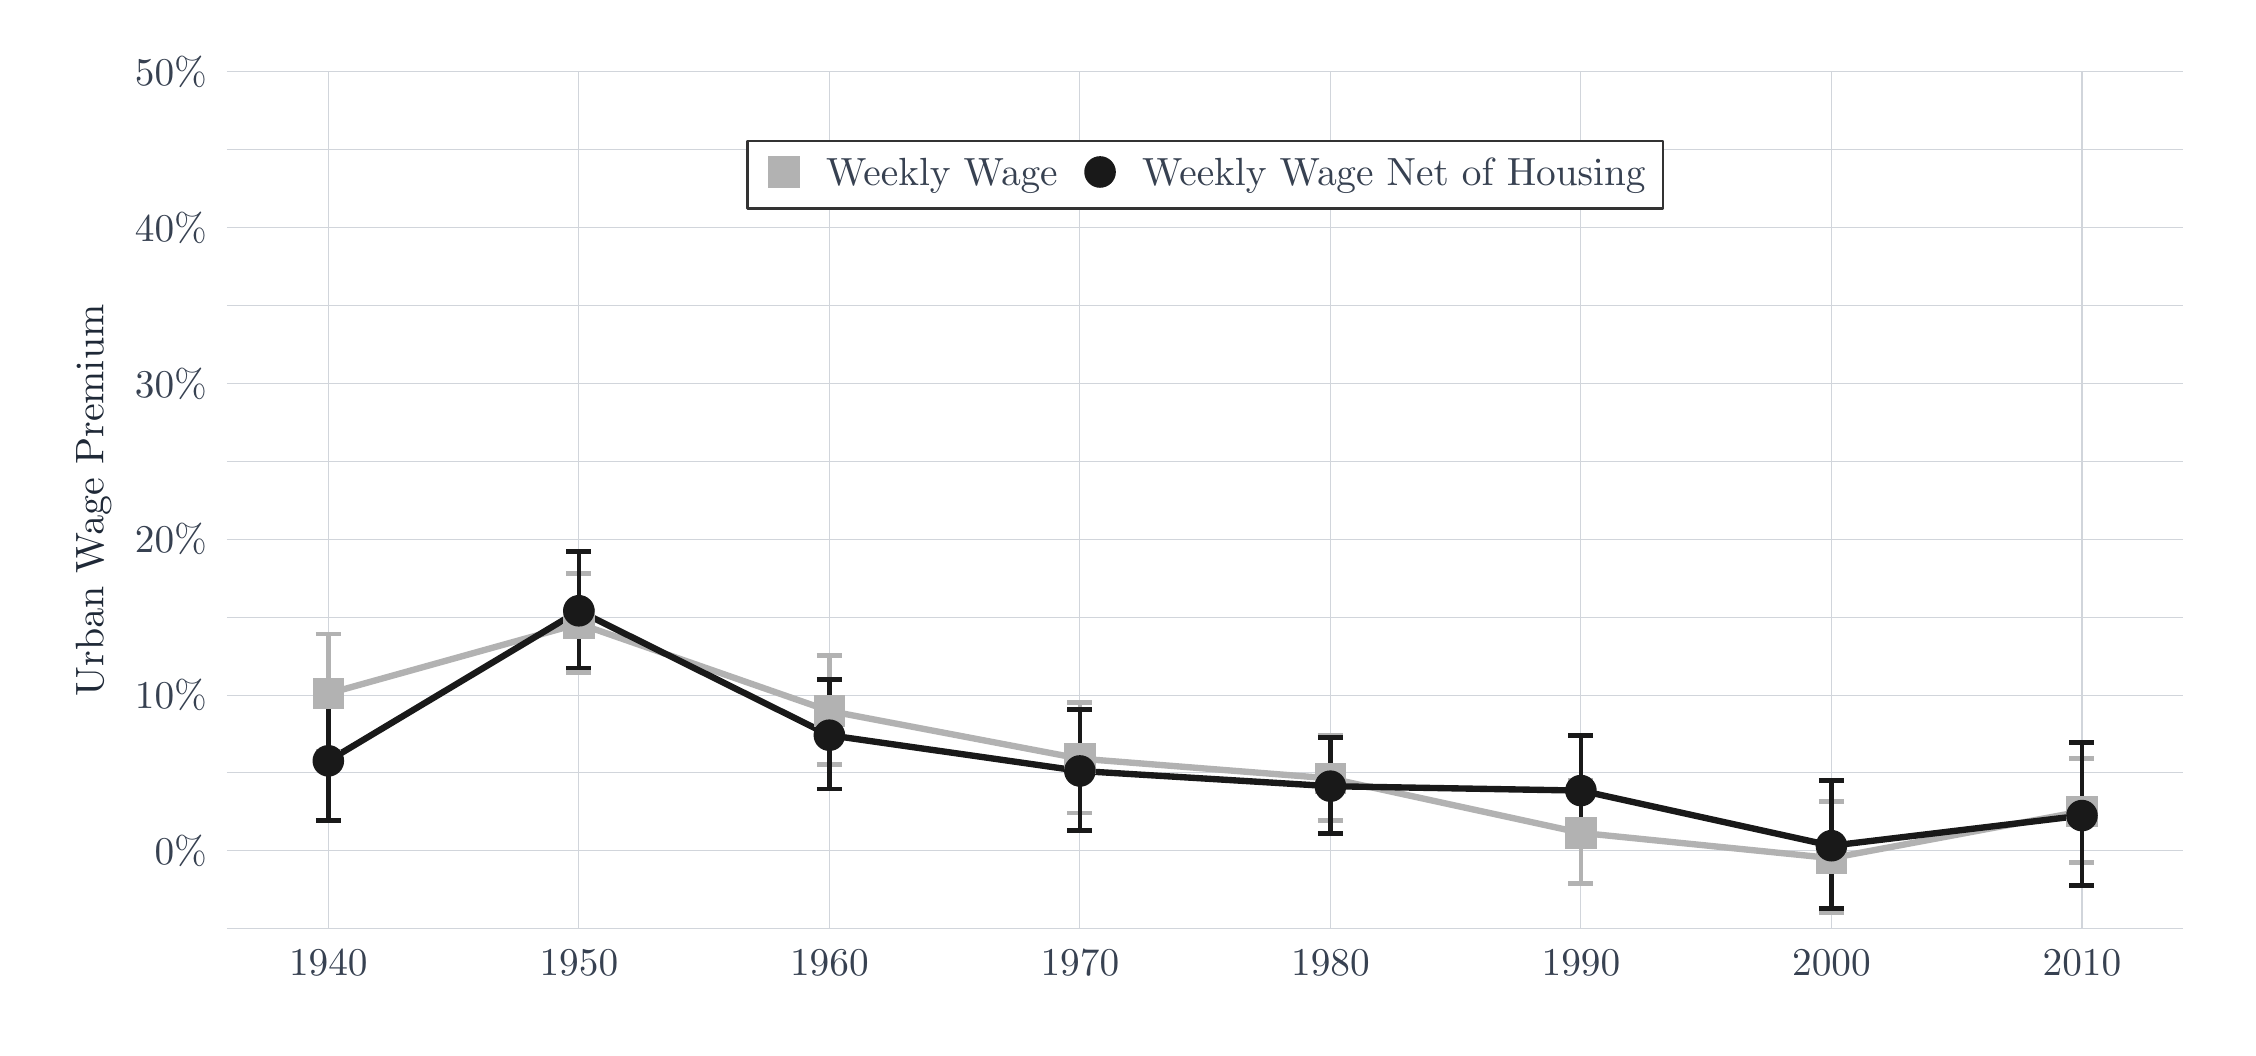
\begin{tikzpicture}[x=1pt,y=1pt]
\definecolor{fillColor}{RGB}{255,255,255}
\path[use as bounding box,fill=fillColor] (0,0) rectangle (794.97,361.35);
\begin{scope}
\path[clip] (  0.00,  0.00) rectangle (794.97,361.35);
\definecolor{drawColor}{RGB}{255,255,255}

\path[draw=drawColor,line width= 0.8pt,line join=round,line cap=round,fill=fillColor] (  0.00,  0.00) rectangle (794.97,361.35);
\end{scope}
\begin{scope}
\path[clip] ( 71.98, 35.76) rectangle (778.97,345.35);
\definecolor{drawColor}{RGB}{255,255,255}
\definecolor{fillColor}{RGB}{255,255,255}

\path[draw=drawColor,line width= 0.8pt,line join=round,line cap=round,fill=fillColor] ( 71.98, 35.76) rectangle (778.97,345.35);
\definecolor{drawColor}{RGB}{209,213,219}

\path[draw=drawColor,line width= 0.4pt,line join=round] ( 71.98, 35.76) --
	(778.97, 35.76);

\path[draw=drawColor,line width= 0.4pt,line join=round] ( 71.98, 92.05) --
	(778.97, 92.05);

\path[draw=drawColor,line width= 0.4pt,line join=round] ( 71.98,148.34) --
	(778.97,148.34);

\path[draw=drawColor,line width= 0.4pt,line join=round] ( 71.98,204.63) --
	(778.97,204.63);

\path[draw=drawColor,line width= 0.4pt,line join=round] ( 71.98,260.92) --
	(778.97,260.92);

\path[draw=drawColor,line width= 0.4pt,line join=round] ( 71.98,317.21) --
	(778.97,317.21);

\path[draw=drawColor,line width= 0.4pt,line join=round] ( 71.98, 63.90) --
	(778.97, 63.90);

\path[draw=drawColor,line width= 0.4pt,line join=round] ( 71.98,120.19) --
	(778.97,120.19);

\path[draw=drawColor,line width= 0.4pt,line join=round] ( 71.98,176.48) --
	(778.97,176.48);

\path[draw=drawColor,line width= 0.4pt,line join=round] ( 71.98,232.77) --
	(778.97,232.77);

\path[draw=drawColor,line width= 0.4pt,line join=round] ( 71.98,289.06) --
	(778.97,289.06);

\path[draw=drawColor,line width= 0.4pt,line join=round] ( 71.98,345.35) --
	(778.97,345.35);

\path[draw=drawColor,line width= 0.4pt,line join=round] (108.64, 35.76) --
	(108.64,345.35);

\path[draw=drawColor,line width= 0.4pt,line join=round] (199.17, 35.76) --
	(199.17,345.35);

\path[draw=drawColor,line width= 0.4pt,line join=round] (289.69, 35.76) --
	(289.69,345.35);

\path[draw=drawColor,line width= 0.4pt,line join=round] (380.21, 35.76) --
	(380.21,345.35);

\path[draw=drawColor,line width= 0.4pt,line join=round] (470.74, 35.76) --
	(470.74,345.35);

\path[draw=drawColor,line width= 0.4pt,line join=round] (561.26, 35.76) --
	(561.26,345.35);

\path[draw=drawColor,line width= 0.4pt,line join=round] (651.78, 35.76) --
	(651.78,345.35);

\path[draw=drawColor,line width= 0.4pt,line join=round] (742.31, 35.76) --
	(742.31,345.35);
\definecolor{drawColor}{gray}{0.70}

\path[draw=drawColor,line width= 2.3pt,line join=round] (108.64,120.74) --
	(199.17,145.98) --
	(289.69,114.44) --
	(380.21, 97.22) --
	(470.74, 90.07) --
	(561.26, 70.39) --
	(651.78, 61.27) --
	(742.31, 78.17);
\definecolor{drawColor}{gray}{0.10}

\path[draw=drawColor,line width= 2.3pt,line join=round] (108.64, 96.42) --
	(199.17,150.64) --
	(289.69,105.68) --
	(380.21, 92.76) --
	(470.74, 87.26) --
	(561.26, 85.67) --
	(651.78, 65.75) --
	(742.31, 76.63);
\definecolor{drawColor}{gray}{0.70}

\path[draw=drawColor,line width= 1.7pt,line join=round] (104.12,142.20) --
	(113.17,142.20);

\path[draw=drawColor,line width= 1.7pt,line join=round] (108.64,142.20) --
	(108.64,100.00);

\path[draw=drawColor,line width= 1.7pt,line join=round] (104.12,100.00) --
	(113.17,100.00);
\definecolor{drawColor}{gray}{0.10}

\path[draw=drawColor,line width= 1.7pt,line join=round] (104.12,118.91) --
	(113.17,118.91);

\path[draw=drawColor,line width= 1.7pt,line join=round] (108.64,118.91) --
	(108.64, 74.76);

\path[draw=drawColor,line width= 1.7pt,line join=round] (104.12, 74.76) --
	(113.17, 74.76);
\definecolor{drawColor}{gray}{0.70}

\path[draw=drawColor,line width= 1.7pt,line join=round] (194.64,164.21) --
	(203.69,164.21);

\path[draw=drawColor,line width= 1.7pt,line join=round] (199.17,164.21) --
	(199.17,128.25);

\path[draw=drawColor,line width= 1.7pt,line join=round] (194.64,128.25) --
	(203.69,128.25);
\definecolor{drawColor}{gray}{0.10}

\path[draw=drawColor,line width= 1.7pt,line join=round] (194.64,171.97) --
	(203.69,171.97);

\path[draw=drawColor,line width= 1.7pt,line join=round] (199.17,171.97) --
	(199.17,129.99);

\path[draw=drawColor,line width= 1.7pt,line join=round] (194.64,129.99) --
	(203.69,129.99);
\definecolor{drawColor}{gray}{0.70}

\path[draw=drawColor,line width= 1.7pt,line join=round] (285.16,134.50) --
	(294.22,134.50);

\path[draw=drawColor,line width= 1.7pt,line join=round] (289.69,134.50) --
	(289.69, 95.01);

\path[draw=drawColor,line width= 1.7pt,line join=round] (285.16, 95.01) --
	(294.22, 95.01);
\definecolor{drawColor}{gray}{0.10}

\path[draw=drawColor,line width= 1.7pt,line join=round] (285.16,125.75) --
	(294.22,125.75);

\path[draw=drawColor,line width= 1.7pt,line join=round] (289.69,125.75) --
	(289.69, 86.25);

\path[draw=drawColor,line width= 1.7pt,line join=round] (285.16, 86.25) --
	(294.22, 86.25);
\definecolor{drawColor}{gray}{0.70}

\path[draw=drawColor,line width= 1.7pt,line join=round] (375.69,117.57) --
	(384.74,117.57);

\path[draw=drawColor,line width= 1.7pt,line join=round] (380.21,117.57) --
	(380.21, 77.54);

\path[draw=drawColor,line width= 1.7pt,line join=round] (375.69, 77.54) --
	(384.74, 77.54);
\definecolor{drawColor}{gray}{0.10}

\path[draw=drawColor,line width= 1.7pt,line join=round] (375.69,115.07) --
	(384.74,115.07);

\path[draw=drawColor,line width= 1.7pt,line join=round] (380.21,115.07) --
	(380.21, 71.26);

\path[draw=drawColor,line width= 1.7pt,line join=round] (375.69, 71.26) --
	(384.74, 71.26);
\definecolor{drawColor}{gray}{0.70}

\path[draw=drawColor,line width= 1.7pt,line join=round] (466.21,105.59) --
	(475.26,105.59);

\path[draw=drawColor,line width= 1.7pt,line join=round] (470.74,105.59) --
	(470.74, 74.95);

\path[draw=drawColor,line width= 1.7pt,line join=round] (466.21, 74.95) --
	(475.26, 74.95);
\definecolor{drawColor}{gray}{0.10}

\path[draw=drawColor,line width= 1.7pt,line join=round] (466.21,104.92) --
	(475.26,104.92);

\path[draw=drawColor,line width= 1.7pt,line join=round] (470.74,104.92) --
	(470.74, 70.11);

\path[draw=drawColor,line width= 1.7pt,line join=round] (466.21, 70.11) --
	(475.26, 70.11);
\definecolor{drawColor}{gray}{0.70}

\path[draw=drawColor,line width= 1.7pt,line join=round] (556.73, 89.22) --
	(565.79, 89.22);

\path[draw=drawColor,line width= 1.7pt,line join=round] (561.26, 89.22) --
	(561.26, 52.15);

\path[draw=drawColor,line width= 1.7pt,line join=round] (556.73, 52.15) --
	(565.79, 52.15);
\definecolor{drawColor}{gray}{0.10}

\path[draw=drawColor,line width= 1.7pt,line join=round] (556.73,105.64) --
	(565.79,105.64);

\path[draw=drawColor,line width= 1.7pt,line join=round] (561.26,105.64) --
	(561.26, 66.36);

\path[draw=drawColor,line width= 1.7pt,line join=round] (556.73, 66.36) --
	(565.79, 66.36);
\definecolor{drawColor}{gray}{0.70}

\path[draw=drawColor,line width= 1.7pt,line join=round] (647.26, 81.81) --
	(656.31, 81.81);

\path[draw=drawColor,line width= 1.7pt,line join=round] (651.78, 81.81) --
	(651.78, 41.45);

\path[draw=drawColor,line width= 1.7pt,line join=round] (647.26, 41.45) --
	(656.31, 41.45);
\definecolor{drawColor}{gray}{0.10}

\path[draw=drawColor,line width= 1.7pt,line join=round] (647.26, 89.38) --
	(656.31, 89.38);

\path[draw=drawColor,line width= 1.7pt,line join=round] (651.78, 89.38) --
	(651.78, 43.07);

\path[draw=drawColor,line width= 1.7pt,line join=round] (647.26, 43.07) --
	(656.31, 43.07);
\definecolor{drawColor}{gray}{0.70}

\path[draw=drawColor,line width= 1.7pt,line join=round] (737.78, 97.29) --
	(746.83, 97.29);

\path[draw=drawColor,line width= 1.7pt,line join=round] (742.31, 97.29) --
	(742.31, 59.67);

\path[draw=drawColor,line width= 1.7pt,line join=round] (737.78, 59.67) --
	(746.83, 59.67);
\definecolor{drawColor}{gray}{0.10}

\path[draw=drawColor,line width= 1.7pt,line join=round] (737.78,103.03) --
	(746.83,103.03);

\path[draw=drawColor,line width= 1.7pt,line join=round] (742.31,103.03) --
	(742.31, 51.38);

\path[draw=drawColor,line width= 1.7pt,line join=round] (737.78, 51.38) --
	(746.83, 51.38);
\definecolor{fillColor}{gray}{0.70}

\path[fill=fillColor] (102.93,115.03) --
	(114.35,115.03) --
	(114.35,126.45) --
	(102.93,126.45) --
	cycle;
\definecolor{fillColor}{gray}{0.10}

\path[fill=fillColor] (108.64, 96.42) circle (  5.71);
\definecolor{fillColor}{gray}{0.70}

\path[fill=fillColor] (193.46,140.27) --
	(204.88,140.27) --
	(204.88,151.69) --
	(193.46,151.69) --
	cycle;
\definecolor{fillColor}{gray}{0.10}

\path[fill=fillColor] (199.17,150.64) circle (  5.71);
\definecolor{fillColor}{gray}{0.70}

\path[fill=fillColor] (283.98,108.73) --
	(295.40,108.73) --
	(295.40,120.15) --
	(283.98,120.15) --
	cycle;
\definecolor{fillColor}{gray}{0.10}

\path[fill=fillColor] (289.69,105.68) circle (  5.71);
\definecolor{fillColor}{gray}{0.70}

\path[fill=fillColor] (374.50, 91.51) --
	(385.92, 91.51) --
	(385.92,102.93) --
	(374.50,102.93) --
	cycle;
\definecolor{fillColor}{gray}{0.10}

\path[fill=fillColor] (380.21, 92.76) circle (  5.71);
\definecolor{fillColor}{gray}{0.70}

\path[fill=fillColor] (465.03, 84.36) --
	(476.45, 84.36) --
	(476.45, 95.78) --
	(465.03, 95.78) --
	cycle;
\definecolor{fillColor}{gray}{0.10}

\path[fill=fillColor] (470.74, 87.26) circle (  5.71);
\definecolor{fillColor}{gray}{0.70}

\path[fill=fillColor] (555.55, 64.68) --
	(566.97, 64.68) --
	(566.97, 76.10) --
	(555.55, 76.10) --
	cycle;
\definecolor{fillColor}{gray}{0.10}

\path[fill=fillColor] (561.26, 85.67) circle (  5.71);
\definecolor{fillColor}{gray}{0.70}

\path[fill=fillColor] (646.07, 55.56) --
	(657.49, 55.56) --
	(657.49, 66.98) --
	(646.07, 66.98) --
	cycle;
\definecolor{fillColor}{gray}{0.10}

\path[fill=fillColor] (651.78, 65.75) circle (  5.71);
\definecolor{fillColor}{gray}{0.70}

\path[fill=fillColor] (736.60, 72.46) --
	(748.02, 72.46) --
	(748.02, 83.88) --
	(736.60, 83.88) --
	cycle;
\definecolor{fillColor}{gray}{0.10}

\path[fill=fillColor] (742.31, 76.63) circle (  5.71);
\end{scope}
\begin{scope}
\path[clip] (  0.00,  0.00) rectangle (794.97,361.35);
\definecolor{drawColor}{RGB}{55,65,81}

\node[text=drawColor,anchor=base east,inner sep=0pt, outer sep=0pt, scale=  1.42] at ( 64.78, 59.01) {0\%};

\node[text=drawColor,anchor=base east,inner sep=0pt, outer sep=0pt, scale=  1.42] at ( 64.78,115.30) {10\%};

\node[text=drawColor,anchor=base east,inner sep=0pt, outer sep=0pt, scale=  1.42] at ( 64.78,171.58) {20\%};

\node[text=drawColor,anchor=base east,inner sep=0pt, outer sep=0pt, scale=  1.42] at ( 64.78,227.87) {30\%};

\node[text=drawColor,anchor=base east,inner sep=0pt, outer sep=0pt, scale=  1.42] at ( 64.78,284.16) {40\%};

\node[text=drawColor,anchor=base east,inner sep=0pt, outer sep=0pt, scale=  1.42] at ( 64.78,340.45) {50\%};
\end{scope}
\begin{scope}
\path[clip] (  0.00,  0.00) rectangle (794.97,361.35);
\definecolor{drawColor}{RGB}{55,65,81}

\node[text=drawColor,anchor=base,inner sep=0pt, outer sep=0pt, scale=  1.42] at (108.64, 18.76) {1940};

\node[text=drawColor,anchor=base,inner sep=0pt, outer sep=0pt, scale=  1.42] at (199.17, 18.76) {1950};

\node[text=drawColor,anchor=base,inner sep=0pt, outer sep=0pt, scale=  1.42] at (289.69, 18.76) {1960};

\node[text=drawColor,anchor=base,inner sep=0pt, outer sep=0pt, scale=  1.42] at (380.21, 18.76) {1970};

\node[text=drawColor,anchor=base,inner sep=0pt, outer sep=0pt, scale=  1.42] at (470.74, 18.76) {1980};

\node[text=drawColor,anchor=base,inner sep=0pt, outer sep=0pt, scale=  1.42] at (561.26, 18.76) {1990};

\node[text=drawColor,anchor=base,inner sep=0pt, outer sep=0pt, scale=  1.42] at (651.78, 18.76) {2000};

\node[text=drawColor,anchor=base,inner sep=0pt, outer sep=0pt, scale=  1.42] at (742.31, 18.76) {2010};
\end{scope}
\begin{scope}
\path[clip] (  0.00,  0.00) rectangle (794.97,361.35);
\definecolor{drawColor}{RGB}{31,41,55}

\node[text=drawColor,rotate= 90.00,anchor=base,inner sep=0pt, outer sep=0pt, scale=  1.44] at ( 27.32,190.55) {Urban Wage Premium};
\end{scope}
\begin{scope}
\path[clip] (  0.00,  0.00) rectangle (794.97,361.35);
\definecolor{drawColor}{gray}{0.20}
\definecolor{fillColor}{RGB}{255,255,255}

\path[draw=drawColor,line width= 0.8pt,line join=round,line cap=round,fill=fillColor] (260.10,295.97) rectangle (590.85,320.43);
\end{scope}
\begin{scope}
\path[clip] (  0.00,  0.00) rectangle (794.97,361.35);
\definecolor{drawColor}{RGB}{255,255,255}
\definecolor{fillColor}{RGB}{255,255,255}

\path[draw=drawColor,line width= 0.8pt,line join=round,line cap=round,fill=fillColor] (266.10,301.97) rectangle (280.55,316.43);
\end{scope}
\begin{scope}
\path[clip] (  0.00,  0.00) rectangle (794.97,361.35);
\definecolor{fillColor}{gray}{0.70}

\path[fill=fillColor] (267.61,303.49) --
	(279.03,303.49) --
	(279.03,314.91) --
	(267.61,314.91) --
	cycle;
\end{scope}
\begin{scope}
\path[clip] (  0.00,  0.00) rectangle (794.97,361.35);
\definecolor{drawColor}{RGB}{255,255,255}
\definecolor{fillColor}{RGB}{255,255,255}

\path[draw=drawColor,line width= 0.8pt,line join=round,line cap=round,fill=fillColor] (380.27,301.97) rectangle (394.72,316.43);
\end{scope}
\begin{scope}
\path[clip] (  0.00,  0.00) rectangle (794.97,361.35);
\definecolor{fillColor}{gray}{0.10}

\path[fill=fillColor] (387.50,309.20) circle (  5.71);
\end{scope}
\begin{scope}
\path[clip] (  0.00,  0.00) rectangle (794.97,361.35);
\definecolor{drawColor}{RGB}{55,65,81}

\node[text=drawColor,anchor=base west,inner sep=0pt, outer sep=0pt, scale=  1.42] at (288.55,304.30) {Weekly Wage};
\end{scope}
\begin{scope}
\path[clip] (  0.00,  0.00) rectangle (794.97,361.35);
\definecolor{drawColor}{RGB}{55,65,81}

\node[text=drawColor,anchor=base west,inner sep=0pt, outer sep=0pt, scale=  1.42] at (402.72,304.30) {Weekly Wage Net of Housing};
\end{scope}
\end{tikzpicture}
